%--------------- Introduction -------------------------
\chapter{Economics Planing In Bangladesh (1972-2022)}
\section{Introduction}
Economic planning plays a crucial role in shaping the development of a nation. 
This assignment delves into the economic planning in Bangladesh over five decades, 
from its liberation war in 1971 to 2022, analyzing the key plans, their execution, 
and assessing their success and failures.


%------------------- The Liberation War Of Bangladesh -----------
\section{The Liberation War Of Bangladesh}
The Liberation War of Bangladesh, which took place in 1971, was a momentous chapter in 
the nation's history. It was a fight for independence, a battle to break free from Pakistan 
and establish Bangladesh as a separate, sovereign country. The people of Bangladesh were driven 
to this struggle because we were being treated unfairly by the government of Pakistan. We wanted 
the right to make our own decisions and govern ourselves. This war was no easy task; it was 
a difficult and challenging period where many people faced hardships and suffering. 
Families were torn apart, and the land bore witness to both heroism and sacrifice.\\

The war, which began on March 26, 1971, was marked by intense fighting and determination. 
Over nine months, the people of Bangladesh, with support from some countries, fought bravely 
for their independence. Finally, on December 16, 1971, the victory was achieved, and Bangladesh 
emerged as an independent nation. This historic day, known as Victory Day, is celebrated every year 
with pride and honor. It signifies the strength, resilience, and the unwavering spirit of 
the Bangladeshi people in their quest for self-determination and freedom. The Liberation 
War is a pivotal event that shaped the identity and history of Bangladesh, and its memory 
continues to be a source of national pride and reflection.


%------------ History of Economics planning in Bangladesh ---------
\section{History of Economics planning in Bangladesh}
Bangladesh, a country in South Asia, has a history of trying to make its economy better. 
It started this journey in 1972 when it became an independent country after a long fight for freedom. 
From then until 2022, Bangladesh has had different plans for its economy. These plans have helped the 
country grow and change.\\

At the start, when Bangladesh was new and had just become a country, the government had to rebuild many things. 
Bangladesh made its first plan in 1973. This plan was like a road map to help develop different parts of 
the country, such as farming, roads, and education. But as time went on, the way Bangladesh planned its economy 
changed. For a while, the country followed a model where the government controlled many businesses. 
This was from 1975 to 1991. The country made different plans during this time, but the government was more 
involved in things like factories and banks.\\

In the 1980s and 1990s, big international groups like the World Bank and the IMF started 
to influence how Bangladesh planned its economy. They wanted the country to open up to 
the world and make changes in how the economy worked. So, Bangladesh started to sell some of 
the businesses it owned and tried to make its economy more like a free market.\\

From 2016 to 2022, Bangladesh started thinking about how to grow in a way that helps 
the environment and its people. The country made the Seventh Five-Year Plan to develop 
the country's infrastructure, make more electricity, and use digital technology to help their economy.\\

This story of Bangladesh's economic planning is a way to see how a country can grow and change over time, 
from a place with lots of problems to a place with big dreams and hopes for the future.



%------------ Time Peiodes of Economics Planning ------------
\subsection{Time Periods of Economic Plans}
Over the 50-year period, several economic plans were implemented. These include:
\begin{enumerate}
	\item The First Five-Year Plan (1973-1978)
	\item The Second Five-Year Plan (1980-1985)
	\item The Third Five-Year Plan (1985-1990)
	\item The Fourth Five-Year Plan (1990-1995)
	\item The Fifth Five-Year Plan (1997-2002)
	\item The Sixth Five-Year Plan (2011-2015)
	\item The Seventh Five-Year Plan (2016-2020)
	\item  Eighth Five-Year Plan (2021-2025)
\end{enumerate}


%----------- Classifications of Bangladesh Economic Structure ---------
\section{Classifications of Bangladesh Economic Plane}
The eight FYPs of Bangladesh can be classified into two broad groups:

\begin{enumerate}
	\item \textbf{Post-war rehabilitation and reconstruction plans (First FYP to Fourth FYP):} 
	These plans focused on rebuilding the economy and infrastructure that had been damaged by the Liberation War.
	\item \textbf{Economic development plans (Fifth FYP to Eighth FYP):} These plans focused on 
	accelerating economic growth and improving the living standards of the people.
\end{enumerate}

\vspace{0.5cm}
\textbf{More details on the eight FYPs}
\begin{enumerate}

	\item\textbf{The First Five-Year Plan (1973-1978)}
	\begin{itemize}
		\item\textbf{Priorities:} Rehabilitation and reconstruction of the economy and infrastructure
		\item\textbf{Key achievements:} Restoration of agricultural production, repair of infrastructure, 
		and provision of basic services
	\end{itemize}
	
	\item\textbf{The Second Five-Year Plan (1980-1985)}
	\begin{itemize}
		\item\textbf{Priorities:} Continued rehabilitation and reconstruction, as well as 
		economic development
		\item\textbf{Key achievements:} Further restoration of agricultural production, 
		expansion of infrastructure, and introduction of policy reforms to promote private 
		sector investment and export-oriented growth
	\end{itemize}
	
	\item\textbf{The Third Five-Year Plan (1985-1990)}
	\begin{itemize}
		\item\textbf{Priorities:} Sustaining economic growth and reducing poverty
		\item\textbf{Key achievements:} High economic growth averaging 7\% per year, 
		significant reduction in poverty rates, and expansion of social services
	\end{itemize}
	
	\item\textbf{The Fourth Five-Year Plan (1990-1995)}
	\begin{itemize}
		\item\textbf{Priorities:} Sustaining economic growth and reducing poverty further
		\item\textbf{Key achievements:} Continued high economic growth, further reduction in 
		poverty rates, and expansion of social services
	\end{itemize}
	
	\item\textbf{The Fifth Five-Year Plan (1997-2002)}
	\begin{itemize}
		\item\textbf{Priorities:} Economic development and poverty reduction
		\item\textbf{Key achievements:} Sustained economic growth averaging 6\% per year, 
		further reduction in poverty rates, and expansion of social services
	\end{itemize}
	
	\item\textbf{The Sixth Five-Year Plan (2011-2015)}
	\begin{itemize}
		\item\textbf{Priorities:} Economic development, social development, and environmental protection
		\item\textbf{Key achievements:} Sustained economic growth averaging 6\% per year, expansion of 
		social services, and increased investment in environmental protection
	\end{itemize}
	
	\item\textbf{The Seventh Five-Year Plan (2016-2020)}
	\begin{itemize}
		\item\textbf{Priorities:} Achieving middle-income country status by 2021
		\item\textbf{Key achievements:} Sustained economic growth averaging 6\% per year, 
		significant progress in achieving middle-income country status, and expansion of social services
	\end{itemize}
	
	\item\textbf{Eighth Five-Year Plan (2021-2025)}
	\begin{itemize}
		\item\textbf{Priorities:} Sustainable and inclusive development
		\item\textbf{Key achievements:} Achieve GDP growth of 8.5\% per year, 
		reduce poverty rate to 7.4\%, and create 13.3 million new jobs
	\end{itemize}
	
\end{enumerate}


%---------- Early Economic Challanges ---------------------------------------
\section{Early Economic Challenges (1972-1980) \& Initial Economic Policies:}

In the early years following its independence in 1971, Bangladesh confronted a multitude 
of formidable economic challenges, primarily stemming from the aftermath of the Liberation War and 
the long-standing disparities between East and West Pakistan. Below, I've outlined the key economic 
challenges and initial economic policies implemented, providing historical context and details.

\begin{enumerate}

	\item\textbf{Infrastructure Rehabilitation}
	\begin{itemize}
		\item\textbf{Challenges:} The Liberation War caused widespread destruction of infrastructure, 
		including roads, bridges, and power facilities.
		\item\textbf{Policies:} The government initiated a comprehensive program to rebuild infrastructure, 
		focusing on repairing roads and bridges, rehabilitating power plants, and restoring communication networks. 
		These efforts were essential for reconnecting regions and revitalizing economic activities.
	\end{itemize}
	
	\item\textbf{War-induced Disruption}
	\begin{itemize}
		\item\textbf{Challenges:} The war disrupted economic activities, 
		causing production stoppages and supply chain breakdowns.
		\item\textbf{Policies:} To address this, the government implemented 
		policies aimed at stimulating economic activities. Incentives were offered to 
		industries and businesses, and local production was encouraged to kick start economic growth. 
		The government also sought foreign aid for reconstruction.
	\end{itemize}
	
	\item\textbf{Resource Constraints}
	\begin{itemize}
		\item\textbf{Challenges:} Bangladesh faced significant resource constraints, 
		including a lack of foreign exchange reserves and capital for investments.
		\item\textbf{Policies:} The government adopted policies to mobilize resources, 
		including negotiations for foreign aid agreements and securing grants and loans 
		from international partners to address resource gaps.
	\end{itemize}
	
	\item\textbf{Food Security}
	\begin{itemize}
		\item\textbf{Challenges:} The war disrupted food production and distribution, leading to severe food shortages.
		\item\textbf{Policies:} Early policies placed a strong emphasis on food security initiatives. 
		Programs were introduced to increase agricultural production, improve food distribution networks, 
		and stabilize food prices, ensuring food security for the population.
	\end{itemize}
	
	\item\textbf{Depleted Treasury}
	\begin{itemize}
		\item\textbf{Challenges:} The national treasury inherited from the Pakistan era was nearly empty, 
		presenting a significant financial challenge.
		\item\textbf{Policies:} To address this challenge, the government explored various avenues for 
		resource generation. This included seeking international financial assistance and improving revenue 
		collection efforts to replenish the treasury.
	\end{itemize}
	
	\item\textbf{Inflation and Price Rises}
	\begin{itemize}
		\item\textbf{Challenges:} The economic turmoil, supply disruptions, and war-induced inflation led 
		to price rises for essential goods.
		\item\textbf{Policies:} Stabilizing prices and controlling inflation were key policy objectives. 
		The government took measures to address price volatility and ensure affordability for the population.
	\end{itemize}
	
	\item\textbf{Humanitarian Crisis}
	\begin{itemize}
		\item\textbf{Challenges:} The war created a massive humanitarian crisis with millions of refugees 
		and internally displaced persons.
		\item\textbf{Policies:} Policies were implemented to address the humanitarian crisis, 
		providing shelter, health-care, and basic necessities to the affected population. 
		International organizations also played a significant role in humanitarian efforts.
	\end{itemize}
	
	\item\textbf{Institutional Building}
	\begin{itemize}
		\item\textbf{Challenges:} Bangladesh had to build its administrative institutions from the ground up, 
		with a lack of experienced bureaucrats.
		\item\textbf{Policies:} Early policies focused on establishing a functional governmental structure, 
		recruiting and training personnel, and creating a framework for governance.
	\end{itemize}
	
	\item\textbf{Reintegration of Returning Refugees}
	\begin{itemize}
		\item\textbf{Challenges:} The return of refugees who had fled to India during 
		the war required careful management.
		\item\textbf{Policies:} The government implemented policies to facilitate 
		the reintegration of returning refugees into society. This included providing housing, 
		livelihood opportunities, and support for rebuilding their lives.
	\end{itemize}
	
	\item\textbf{Stimulating Industry and Agriculture}
	\begin{itemize}
		\item\textbf{Challenges:} Reviving the industrial and agricultural sectors was pivotal 
		for economic recovery.
		\item\textbf{Policies:} The government encouraged investment in these sectors, 
		provided incentives for production, and implemented land reforms to promote 
		agriculture and increase food production.
	\end{itemize}
	
\end{enumerate}


%------- Economic Structure of Bangladesh -------------
\section{Economic Structure of Bangladesh}
The economic structure of Bangladesh can be divided into the following three sectors:

\begin{itemize}
	\item\textbf{ Primary Sector: }
	With 45\% of the workforce engaged in the primary sector (est. 2011), Bangladesh can be called 
	an agrarian economy. Agriculture contributes 30\% of the country's GDP and enables Bangladesh 
	to achieve its macroeconomic objectives, including food security, poverty alleviation, human 
	resources development and employment generation. Cooperatives are increasingly motivating farmers 
	to employ modern machinery. Bangladesh primarily produces Jute, Rice, Tobacco, Tea, Sugarcane, 
	Pulses and Wheat. According to the composition of sub sectors, the crop sector contributes 72\% of 
	the production, followed by Fisheries at 10.33\%, livestock at 10.11\% and forestry at 7.33\%. 
	The unpredictable weather and natural calamities disrupt the country's economy frequently. 
	To overcome this problem, the government has several irrigation projects to conserve rainwater 
	and control floods. The projects also include controlling pests and using high quality seeds. 

	\item\textbf{Secondary Sector: }
	This sector mainly comprises of small and medium enterprises that give employment to 30\% of 
	the country's workforce (est. 2011). It generates 25\% of the GDP and 40\% of the gross 
	manufacturing output. Bangladesh's light engineering sector is one of the largest and most diverse, 
	producing a wide variety of machinery and spare parts. There are several mills and factories, 
	producing jute, garments, cotton, paper, textile, pharmaceuticals and fertilizers, 
	among other things. Some major manufacturing industries are railways, tea plantation \& processing 
	industries, construction sector, ferry and transport. Infrastructure is developing swiftly 
	in terms of water distribution, power supply, communications and transportation. 
	Bangladesh features a prominent wealth of coal mines. 
 
 \item\textbf{Tertiary Sector: }
 In the last two decades, Bangladesh has seen incredible growth in its service sector. 
 As of 2011, 25\% (2011 est.) of the country's workforce was employed in this sector. 
 Although this percentage is lesser than the primary and secondary sectors, 
 a large part of the country's GDP comes from service sector. The hospitality industry, in particular, has shown considerable growth.

\end{itemize}

\textbf{Source :}\url{https://www.academia.edu/7983766/Economic_Structure_of_Bangladesh}

\subsection{Overview of Bangladesh Economy}

\begin{table}[h!]
\renewcommand{\arraystretch}{1.7} % Adjust the value to increase cell height
\caption{\textbf{Per capita GDP and GNI at Current Prices}}
\label{table:1}
\begin{tabular}{l l r r r r}
	\bottomrule
	\rowcolor{gray!30}
	\textbf{(Base: 2015-16)} & Unit & 2019-20 & 2020-21 & 2021-22 & 2022-23(p)\\
	\toprule
	GDP 				& (Mill.Tk.) 	& 31,704,694		& 35,301,848 	& 39,717,164 	& 44,392,733 \\
	GNI 				& (Mill.Tk.) 	& 33,017,012		& 37,159,966 	& 41,290,624 	& 46,185,291 \\
	Population 		& (Mill.No.) 	& 167.4 			& 169.11 		& 171.30 		& 170.79 \\
	Per capita GDP 	& (In Tk.) 		& 189,361 		& 208,751 		& 231,861 		& 259,919 \\
	Per capita GNI 	& (In Tk.) 		& 197,199 		& 219,738 		& 241,047 		& 270,414 \\
	Exchange rate 	& (Tk per US\$)	& 84.78 			& 84.81 			& 86.30 			& 97.81 \\
	GDP				& (Mill. US\$) 	& 373,959 		& 416,264 		& 460,219 		& 453,852 \\
	GNI 				& (Mill. US\$) 	& 389,438 		& 438,175 		& 478,451 		& 472,178 \\
	Per capita GDP 	& (In US \$) 	& 2,234 			& 2,462 			& 2,687 			& 2,657 \\
	Per capita GNI 	& (In US \$) 	& 2,326 			& 2,591 			& 2,793 			& 2,765 \\
	\bottomrule
\end{tabular}
\end{table}

\vfill
Source: \url{https://bbs.gov.bd/site/page/b588b454-0f88-4679-bf20-90e06dc1d10b/-}

\newpage
\begin{figure}[h!]
    \centering
    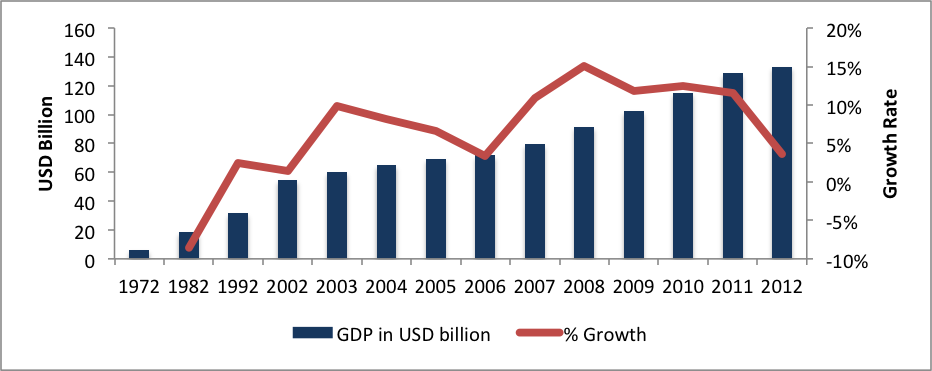
\includegraphics[width=1.00\textwidth]{Figs/GDP.png}
    \caption{ GDP Growth rate of Bangladesh}
    \label{fig:mesh1}
\end{figure}

\vspace{1.3cm}

\begin{figure}[h!]
    \centering
    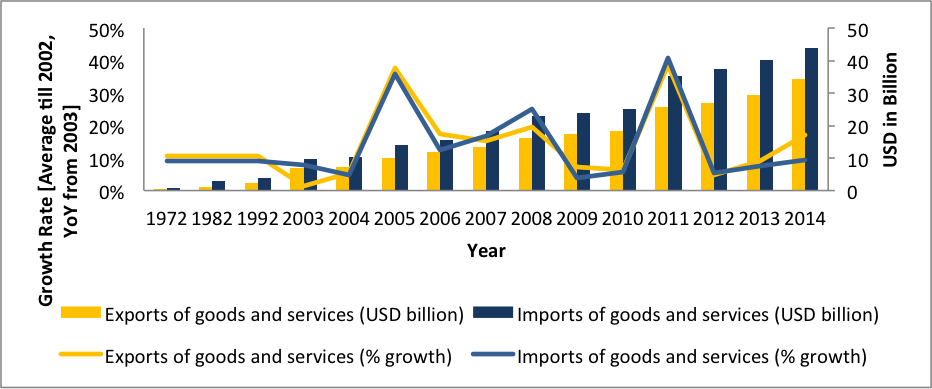
\includegraphics[width=1.00\textwidth]{Figs/TG.png}
    \caption{Trade Growth of Bangladesh}
    \label{fig:mesh1}
\end{figure}

\vfill

\textbf{Source} Embassy of Bangladesh Paris \\ \url{https://www.bangladoot-paris.org/2013-06-03-11-28-34/economy.html}

\begin{figure}[h!]
    \centering
    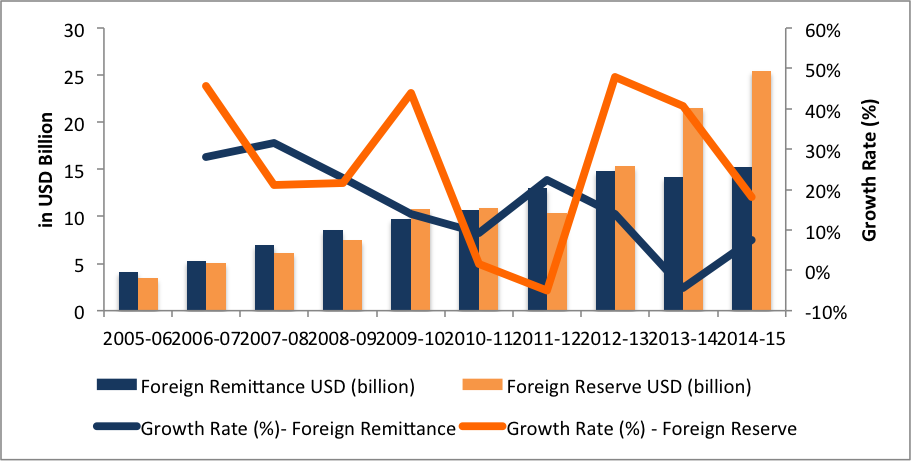
\includegraphics[width=1.00\textwidth]{Figs/FRRG.png}
    \caption{Foreign Reserve and Remittance Growth in Bangladesh}
    \label{fig:mesh1}
\end{figure}

\vspace{1cm}

\begin{figure}[h!]
    \centering
    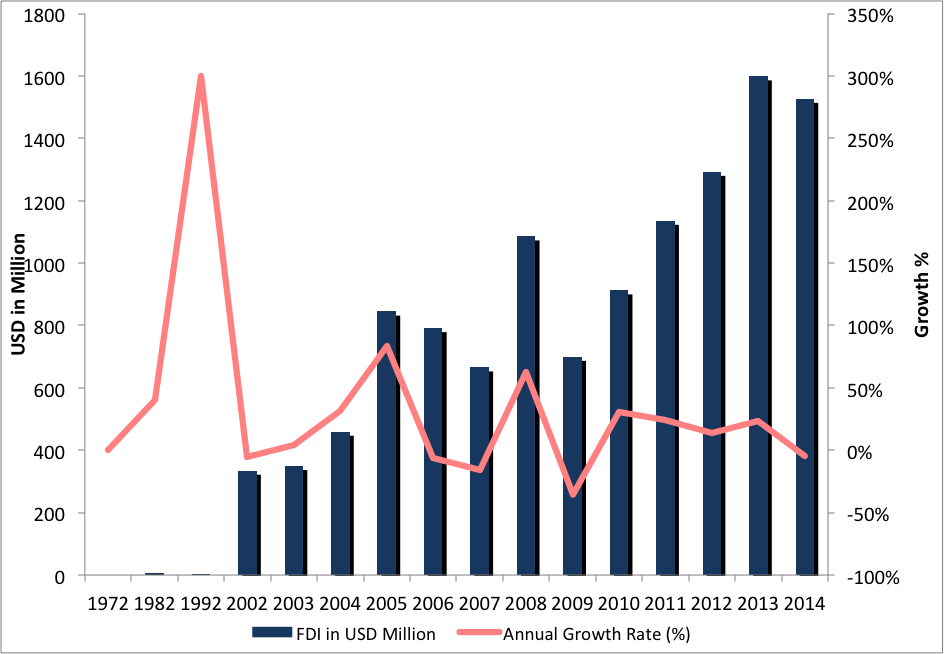
\includegraphics[width=1.00\textwidth]{Figs/FDI.png}
    \caption{ Foreign Direct Investment in Bangladesh}
    \label{fig:mesh1}
\end{figure}


%------- Success and Failure -------------
\newpage
\section{Success and Failure of The Bangladesh Economic Planning}

\subsection{First Five Years Plan (1973-1978)}
After independence of Bangladesh, introduction of socialistic economy received priority to
the policy makers of the government and encouraged the private entrepreneurs for establishing 
new industries along with the nationalized enterprises to get rid of the economic depression. 
To achieve this, this five years plan was prepared.

\begin{itemize}
	\item\textbf{Objectives}
	\begin{itemize}
		\item Reconstruction and Rehabilitation
		\item Agricultural Self-Sufficiency
		\item Employment Generation
		\item Poverty Alleviation
		\item Infrastructure Development
		\item Industrialization
		\item Education and 
		\item Institutional Strengthening
		\item Social Equity
		\item Natural Resource Management
	\end{itemize}

	\item\textbf{Efficiency and Success}
	\begin{itemize}
		\item\textbf{Agricultural Growth: } The plan successfully increased agricultural production, 
		making Bangladesh self-sufficient in food, particularly in rice and wheat. This achievement 
		significantly improved food security.
		\item\textbf{Infrastructure Development: } The plan invested in critical infrastructure projects, 
		including roads, bridges, and irrigation systems, which greatly enhanced transportation and connectivity, 
		improving access to remote areas.
		\item\textbf{Reduced Poverty: } The plan's emphasis on rural development and agriculture 
		contributed to a reduction in rural poverty rates, benefiting a large portion of the population.
		\item\textbf{Expansion of Education: } Efforts to expand educational opportunities led to 
		increased enrollment in schools and a significant rise in literacy rates.
		\item\textbf{Health-care Services: } The plan improved access to basic health-care services, 
		resulting in better health outcomes and a decline in mortality rates, particularly among children.
		\item\textbf{Export Diversification: } It laid the foundation for diversifying exports by promoting 
		non-traditional export items, reducing dependence on a few commodities, and expanding foreign exchange earnings.
		\item\textbf{Employment Generation: } The plan created employment opportunities, especially in the 
		agricultural and rural sectors, helping to alleviate unemployment and underemployment.
		\item\textbf{Institutional Capacity Building: } The plan strengthened government institutions and 
		administrative capacities, enhancing their ability to plan and implement development projects effectively.
		\item\textbf{Regional Development: } It worked to reduce regional disparities 
		by focusing on equitable resource allocation and development across different regions of the country.
	\end{itemize}
	
	\item\textbf{Limitations and Failure}\\
	The government had to face the following hazards in implementing various programs taken 
	in the \textit{First Five Years Plan}.
	\begin{itemize}
		\item Firstly, the expected amount of foreign assistance from the donors could 
		not be received due to unusual inflation and economic meltdown in the developed 
		countries and this situation prolonged up to 1978.
		\item Secondly, devastating flood of 1974 caused massive damage of crops in 
		many years which resulted in famine countrywide.
		\item Thirdly, the export-import ratio of Bangladesh gradually deteriorated 
		in the global market specially the import value of oil increased manifold.
		\item Fourthly, the rehabilitation program management of trade and commerce, 
		finance and industry and building a national administrative structure in a 
		newly born war-ravaged country become very complicated and time consuming.
	\end{itemize}
	
All these reasons delayed and made the rehabilitation task of the economy difficult and pushed back 
the national productivity rate in 1975-1976 to that of 1969-1970
	
\end{itemize}

\subsection{Two Years Plan (1978-1980)}
At the terminal period of the FFYP although overall management of the economy marked
improvement with more stability, objectives of the plan were hindered of too due to many
number of income projects. For this reason, The Second Five Years Plan (SFYP) of the
country could not be formulated. In this situation, a two year plan was formulated to complete
the on-going projects as many as possible within available resources.\\

This plan was instituted to address an economic crisis, fiscal deficits, and balance of
payments challenges, with a focus on immediate policy reforms and structural adjustments
to stabilize the economy and manage limited resources effectively


\subsection{Second Five Years Plan (1980-1985)}
After immediate Completion of the TYP, the Second Five Years Plan(SFYP) was announced
with the programs of attaining the food self-sufficiency, rise of industrial production, 
extended education program and expansion of foreign trade and exchange by exporting man power.

\begin{itemize}
	
	\item\textbf{Objectives}
	\begin{itemize}
		\item Raising the standard of living at noticeable level by 
		ensuring adequate supply of basic needs
		\item Attaining self-sufficiency in the shortest time
		\item Increasing opportunities of productive employment
		\item Eradicating illiteracy through implementation of mass primary education
		\item Reducing Population Growth Rate
		\item Encouraging people's participation in development activities
		\item Utilizing domestic resources
	\end{itemize}
	
	\item\textbf{Efficiency and Success}
	\begin{itemize}
		\item The Economic Growth was strong and consistent, fostering increased
		 stability and development.
		\item Agricultural Productivity was in notable growth, particularly food 
		grains, improved food security and reduced import dependency.
		\item Prioritization of Infrastructure Projects, such as transportation and 
		energy, promoted economic development and accessibility.
		\item By diversifying export items, reliance on a few commodities were reduced 
		and foreign exchange earnings were broadened.
		\item Investments in Education and Health-care improved literacy rates, school 
		enrollments, and health-care services, thereby enhancing the quality of life.
	\end{itemize}
	
	\item\textbf{Limitations and Failure}
	The plan struggled with foreign exchange shortages, affecting the import of essential goods 
	and machinery, which hindered industrial development. Despite an emphasis on industrialization, 
	the plan faced slow industrial growth in the industrial sector, which limited diversification. 
	The plan did not significantly address income inequality, as wealth distribution remained uneven, 
	particularly in rural areas. The rapid population growth rate during the plan period exerted 
	pressure on resources and services, impacting development efforts. For the inflationary pressures, 
	partly due to global oil price increases, affecting the cost of living and the purchasing power of 
	citizens. Political instability disrupted policy implementation and development efforts.	
	
\end{itemize}

\subsection{Third Five Year Plan (1985-1990)}
In the backdrop of internal financial instability, two successive devastating floods, 
protectionism, frequent fluctuations in the trade conditions, unstable aid commitment 
combined with external obstacles; the TFYP was formulated with the expectation of 
creating a stable economic environment in the country.

\begin{itemize}
	\item\textbf{Objectives}
	\begin{itemize}
		\item Reduce the Population Growth Rate
		\item Widen the scope of productive employment
		\item Develop technological base for long-term structural change
		\item Achieve self sufficiency in food
		\item Meet the minimum basic needs of the people
		\item Strengthen Economic Growth
		\item Expedite self reliance
	\end{itemize}
	
	\item\textbf{Efficiency and Success}
	\begin{itemize}
		\item Sustainable contribution in the Economic Growth, 
		with an increased Gross Domestic Product (GDP) and improved economic stability.
		\item Continued to prioritize Infrastructure Development, leading to the expansion 
		of transportation networks, energy supply, and communication systems, which fostered economic progress.
		\item Successful Diversification of Export Items, reducing the country's reliance on 
		a few commodities and broadening foreign exchange earnings.
		\item Encouraging Private Sector Development led to increased investments, 
		job creation, and economic diversification.
		\item Notable improvements in Education and Health-care Services, with increased school enrollments, 
		higher literacy rates, and enhanced health-care accessibility.
	\end{itemize}
	
	\item\textbf{Limitations and Failure}
	Encountering Fiscal Deficits and challenges in revenue collection, impacting the government's 
	ability to fund development projects effectively. No significant development in income inequality, 
	as wealth distribution remained uneven, particularly in rural areas. Rapid Population Growth 
	continued to exert pressure on resources and services, impacting development efforts and social indicators.
	Faced Resource Constraints, affecting the timely implementation of key projects and programs.
	Also faced Inflationary Pressures, partly due to global oil price increases, affecting the cost
	of living and the purchasing power of citizens. Political Instability remains to hinder the development efforts.
	
\end{itemize}


\subsection{Fourth Five Years Plan (1990-1995)}
Average GDP growth during the Fourth Five Years Plan (FFYP) was targeted as at 5\% per
annul,out of which 3.6\% in agriculture, 9.1\% in industry, 11\% in electricity, gas and natural
resources, 8.8\% in construction, 5.4\% in transport and communication, 5.1\% in trade and
others and 3.1\% in public services.

\begin{itemize}
	\item\textbf{Objectives}
	\begin{itemize}
		\item Accelerating Economic Growth. It is envisaged that the Annual Growth Rate of GDP 
		would be 5\% during the plan period
		\item Poverty alleviation and employment generation through human resource development
		\item Increase self-reliance
	\end{itemize}
	
	\item\textbf{Efficiency and Success}
	\begin{itemize}
		\item Continued to robust Economic Growth, fostering economic stability and development, 
		with a consistently increasing Gross Domestic Product (GDP).
		\item Gradual improvement in Infrastructure Development and Human Development which enhanced 
		economic accessibility and quality of life for citizens.
		\item Private Sector Development was growing as the foundation of the economy, as 
		the investment and job creation were going up.
		\item Declination in Poverty Rates were noticed, particularly in rural areas.
		\item Efforts to expand the Energy Sector led to increased energy supply, enhancing energy security
	\end{itemize}
	
	\item\textbf{Limitations and Failure}
	External Factors, such as global economic conditions and international commodity prices, 
	had an impact on the plan’s effectiveness, influencing trade balances and economic stability. 
	Corruption and Governance issues affect the efficient allocation of resources and 
	the implementation of development projects. In spite of improving the infrastructures, 
	there were still Infrastructure Gaps in critical structure of rural areas.
	Although a number of school enrollments were increasing, the Education Quality, 
	particularly in rural areas, remained a concern. Efforts to address Environmental Sustainability 
	were insufficient, with concerns about deforestation and pollution persisting.
\end{itemize}


\subsection{Fifth Five Years Plan (1997-2002)}
The Fifth Five years Plan was formulated keeping in mind a set of dimensions like certain
creation of productive employment and poverty alleviation, self reliance in food, development
of human resources, infrastructures, controlling population growth, maintaining social peace,
getting technology-based knowledge and improvement of social justice etc.

\begin{itemize}
	\item\textbf{Objectives}
	\begin{itemize}
		\item Alleviating poverty(7.3\% per annul) through bringing economic dynamism
		\item Generating ample scope of employment by utilizing labor intensive technology
		\item Achieving food production beyond the self-sufficiency level to export
		\item Taking measures for producing high valued export commodities
		\item Developing necessary infrastructure, private sector and exploration of natural energy
		\item Developing human resources with emphasis on compulsory primary education and vocational training
		\item Keeping Population Growth Rate within 1.20\% by the end of the plan period and 
		ensuring good health and nutrition of babies and mothers
		\item Strengthening country's scientific and technological based with the emphasis on research 
		and development of technologies
		\item Promoting natural resources for sustainable development
		\item Reducing gender gap and supporting girl's education, employment and special support
		\item Establishing social justice by strengthening law and order and the rule of law
	\end{itemize}
	
	\item\textbf{Efficiency and Success}
	\begin{itemize}
		\item Fostering Economic Prosperity, with the country experiencing sustained economic 
		growth and positive trends in its overall economic performance.
		\item A significant emphasis on the Infrastructure Expansion, such as roads, energy supply, 
		and communication systems, leading to improved accessibility and enhancing economic development.
		\item Encouragement of Private Sector initiatives resulted in increased investments and job creation, 
		contributing to economic diversification and expansion.
		\item Modernization of Key Sectors like agriculture, industry, and social services were more efficient, 
		competitive, and in line with contemporary standards.
		\item Increasing literacy rates, and improved access to health-care for the Human Development.
		\item Successful Diversification of Export Items reduced dependency on a limited range of commodities.
	\end{itemize}
	
	\item\textbf{Limitations and Failure}
	Grappling with Resource Limitations, both in terms of financial and human resources. This constrained the 
	comprehensive implementation of development programs and projects, leading to delays and incomplete 
	achievement of various plan objectives. Income Inequality remains one of the persistent failures as 
	the plan did not adequately rectify wealth disparities, particularly in rural areas. Lack of sufficient 
	attention remained a concern about the Long-term Sustainability of development efforts.The rapid and 
	unchecked Population Growth led to the challenges in improving human development indicators. 
	Governance and Corruption including inefficiencies in resource allocation and project implementation, 
	persisted as significant limitations, hindering the full realization of the plan's potential like before.
\end{itemize}

\newpage
\subsection{Sixth Five Years Plan (2011-2015)}
The Sixth Five Years Plan has been made with some core targets in the context of Vision
2021. Notwithstanding past progress with poverty reduction, the Government recognizes
that Bangladesh is still a low income developing country. An estimated 47 million people are
living below the poverty line. Most of the labor force is engaged in low productivity and
low income jobs. The access to secondary and tertiary education is limited and the quality of
education at all levels is deficient. The poor group in Bangladesh is severely disadvantaged
in terms of ownership of assets and has inadequate access to institutional finance as well
as to basic services including quality education, health-care, water and sanitation.This group
of people is also disproportionately affected by natural disasters and the adverse effects of
climate change. Publicly supported mitigating measures in the form of social protection
programs are inadequate

\begin{itemize}
	\item\textbf{Objectives}
	\begin{itemize}
		\item Acceleration of Economic Growth and Employment
		\item Benefiting from higher labor force growth(the demographic dividend) and 
		ensuring \textit{Labor Quality}
		\item Improving factor productivity through \textit{Information Technology}
		\item Reducing \textit{Population Growth}
		\item Ensuring \textit{Food Security}, \textit{Social Protection} for under-privileged 
		population, \textit{Gender Parity} and \textit{Environmental Sustainability}
		\item Improving Governance and Administrative Capacity
		\item Managing the spatial dimensions of growth and reducing
		\item Strengthening \textit{Civil Service}, \textit{Income Inequality}
	\end{itemize}
	
	\item\textbf{Efficiency and Success}
	\begin{itemize}
		\item Growth of Income has gone up from 6.3\% to 7.06\%. This was a substantial 
		growth and highest achievement of GDP in the last 8 years.
		\item As Poverty was the single most important socio-economic policy challenge for Bangladesh, 
		the government was trying hard to reduce the incidence of poverty and improve 
		the living standards of its millions of impoverished citizens. Bangladesh has made 
		substantial progress in reducing poverty, where the percent of population living below 
		the poverty line went down from more than 80 percent in early 1970s to 24.3\% percent in FY10.
		\item Achieving 100 percent net enrollment rate for Primary Education, increasing enrollment 
		rate to 60\% in 12th class and reduced Fertility Rate to 2.2\%
		\item Proportion of rural population with access to safe drinking water increased to 96.5\% 
		and urban population with access to Sanitary Latrines to 100\%.
		\item Generation of Electricity was increased to 15,457 MW by FY15, electrical coverage 
		increased to 68\%, Energy Efficiency by 10\% and development of many critical Infrastructure.
		\item Female to male Ratio in tertiary education to be raised from current 32\% to 60\%.
		\item Environmental Sustainability robust as productive forest coverage increased by 2\%, 
		improving air quality in Dhaka, treated all urban waste in rivers and many other things.
		\item Developing in the ICT sector, increasing public spending on Research and Development 
		to 1\% of GDP by FY15.
	\end{itemize}
	
	\item\textbf{Limitations and Failure}
	Economic Growth was not still sufficient in context of other mid-income country. Sector, Macroeconomic, 
	Urban and Human Resource Development were still need an improvement. And also Gender equality, 
	income inequality, social protection to be improved.
\end{itemize}

\vspace{0.2cm}

\subsection{Seventh Five Years Plan (2016-2020)}

\begin{itemize}
	\item\textbf{Objectives}
	\begin{itemize}
		\item Growth of Income and Reduction of Poverty
		\item Sectoral Development
		\item Human Resource Development
		\item Gender and Income Inequality, Social Protection
		\item Energy and improvement of Infrastructure
		\item Environmental Sustainability
	\end{itemize}		
	
	\item\textbf{Efficiency and Success}
	\begin{itemize}
		\item Attaining average real GDP growth rate of 7.4\% per year and extreme poverty reduced by about 4\%.
		\item Significant growth in the agriculture, industry and service sectors. Also the GDP increased by 21\% 
		for the contribution of the manufacturing sector.
		\item Building Inclusive house for urban inhabitants including for people living in informal settlements and slums.
		\item Installing generation capacity of electricity which was increased to 23,000 MW by 2020 and many other 
		infrastructure to cope up with traffic jam.
		\item Environmental, Climate Change and Disaster Risk Reduction Considerations are integrated into project design, 
		budgetary allocations and implementation process.
		\item Also the notable improvement in ICT Sector.
	\end{itemize}
	
	\item\textbf{Limitations and Failure}
	Poverty was still need to be fully eliminated and more contribution was needed to our GDP. 
	Bangladesh did not attain Upper Middle-Income Country (UMIC) status yet and also major 
	Sustainable Development Goal(SDG) targets. The citizens were not fully benefited by the planning.
\end{itemize}




%---------- 8th Five Year Pla (2020-2025) -------------
\subsection{The Running($8^{th}$) Five Years Plan(2020-2025)}
\textbf{Addressing COVID-19 Challenges and Sustainable LDC Graduation}
\subsubsection{Introduction}
\begin{itemize}
	\item The Eighth Five Year Plan ($8^{th}$ \textit{FYP}),which will be implemented during 
	\textit{FY 2021-25}, is currently being finalized before placing it to the \textit{NEC} for final approval
	\begin{itemize}
		\item The draft plan document, which was prepared early, had to be revisited on account 
		of adjustment because of the \textit{COVID-19} pandemic
	\end{itemize}
	
	\item The $8^{th}$ \textit{FYP} is expected to take into cognizance the experiences and lessons 
	learnt from the $7^{th FYP}$ (\textit{FY 2016–20})
	\begin{itemize}
		\item The experience and result of implementing the $7^{th}$ \textit{FYP} have been rather mixed. 
		The \textit{COVID-19} pandemic has caused major disruptions in macroeconomic management as 
		the plan period reached its final year in \textit{FY2020}
	\end{itemize}
	
	\item The $8^{th}$ \textit{FYP} will need to be informed by three key challenges
	\begin{itemize}
		\item Economic recovery and rebound in \textit{post-COVID} period
		\item Graduation from the LDC group by 2024
		\item Second crucial (five-year) lap in implementing the SDGs by 2030
	\end{itemize}
	
	\item $8^{th}$ \textit{FYP} must also address electoral pledges of the ruling 
	party made prior to 2018 National Election
	
\end{itemize}


\subsubsection{Two broad themes of the plan}
\begin{itemize}
	\item\textbf{Promoting Prosperity}\\
	The plan has emphasized on appropriate policies, frameworks and devised 
	suitable and sustainable development strategies for promoting prosperity. 
	For this, the first step is to bring Bangladesh closer to attaining 
	Upper Middle-income Country (UMIC) status, major Sustainable Development Goal (SDG) 
	targets, and eliminating extreme poverty.
	
	\item\textbf{Fostering Inclusivity}\\
	A broad-based strategy of inclusiveness with a view to empowering every citizen 
	to participate fully and benefit from the development process and helping the poor and 
	vulnerable with social protection- based income transfers has been adopted in the plan.
\end{itemize}

\subsubsection{Plan is divided into two main parts}
\begin{itemize}
	\item\textbf{Macroeconomic perspective}\\
	The first part delineates the macroeconomic framework for the plan period 
	(July 2020-June 2025) along with strategic directions and policy framework 
	for promoting inclusiveness, reducing poverty and inequality. It also describes 
	the resource envelop and overall fiscal management tools of the government 
	and specifies the Development Results Framework (DRF) for proper monitoring and evaluation.
	
	\item\textbf{Sectoral Strategies}\\
	The second part sets out the sectoral strategies for thirteen sectors (except defense) 
	with some specific targets to attain by FY 2025. The ministries/divisions are expected 
	to follow these sectoral strategies and action measures while preparing their sector 
	specific projects and programs to achieve their respective targets set in the $8^{th}$ Five Year Plan.
\end{itemize}

\subsubsection{The $8^{th}$ Plan centers on six sub-core themes}
\begin{enumerate}
	\item \textbf{Rapid recovery from \textit{COVID-19}} to restore human health, confidence, 
	employment, income and economic activities
	
	\item A broad-based \textbf{strategy of inclusiveness} with a view to empowering every citizen 
	to participate fully and benefit from the development process and helping the poor and 
	vulnerable with social protection- based income transfers
	
	\item \textbf{GDP growth acceleration}, employment generation, productivity acceleration 
	and rapid poverty reduction
	
	\item A \textbf{sustainable development} pathway that is resilient to disaster and climate change, 
	entails sustainable use of natural resources and successfully managing the inevitable 
	urbanization transition
	
	\item Development and improvement of critical institutions necessary to 
	\textbf{lead the economy to UMIC status}
	
	\item \textbf{Attaining SDG targets} and coping up the impact of Least Developed Country (LDC) 
	graduation (sustainable transition with exploring alternatives to the erosion of preferential 
	benefits and not to go back to previous LDC status).
	
\end{enumerate}

\begin{table}[h!]
\renewcommand{\arraystretch}{1.5}
\centering
\caption{GDP Growth Projections under the 8FYP}
\label{Table-2}
\begin{tabular}{ p{3cm} p{1.5cm} p{1cm} p{1.3cm} p{1.3cm} p{1.3cm} p{1.3cm}}
\bottomrule
\rowcolor{gray!30}
Particulars & \centering{FY20 (Actual)} & FY21 & FY22 & FY23 & FY24 & FY25 \\
\toprule
Pre-COVID-19 GDP growth (as perpp2041) 	& 8.19	& 8.23	& 8.29	& 8.32	& 8.37	& 8.51 \\
\midrule
GDB growth with COVID-19					& 5.24	& 7.40	& 7.70	& 8.00	& 8.32	& 8.51 \\
\bottomrule
\end{tabular}
\end{table}


\subsubsection{Challenges in implementations of the plan}
During the implementation period of the 8FYP, the government will face a
number of challenges. The \textbf{four} specific ones are the following:
\begin{itemize}
	\item Covid-19 pandemic
	\item Graduation from the least developed country (LDC) category
	\item Implementation of the Sustainable Development Goals (SDGs) and
	\item Climate change vulnerability
\end{itemize}
Besides, Russia Ukraine war, rise in fuel price, disruption in supply chain
and currency devaluation are some other major challenges that government
needs to confront with.

\subsubsection{Focus of the Plan}
\textbf{The plan mainly focuses on 7 areas:}
\begin{enumerate}
	\item Labour-intensive manufacturing
	\item Export-oriented manufacturing-led growth
	\item Agricultural diversification
	\item Dynamism in cottage, small and medium enterprises
	\item Modern services sector
	\item ICT based entrepreneurship, and
	\item Overseas employment.
\end{enumerate}

\subsubsection{8FYP targets for indicators:}
\begin{itemize}
	\item Inflation - 4.60\%
	\item Public \& Private Investment – Public (25.3\%) \& Private (74.7\%)
	\item Employment - 1 corer 13 lac 30 thousands
	\item Poverty reduction – 15.60\%
	\item Revenue mobilization – 12.3\% of GDP
	\item Allocation for Annual Development Plan (ADP) – 3675.3 Billion USD
\end{itemize}

\subsubsection{Key Takeaways}
\begin{itemize}
	\item Bangladesh has targeted 8.51 per cent economic growth for the 8th Five Year Plan. 
	To accommodate this growth target, the gross investment needs to be raised to 36.59 per cent 
	of GDP by FY 2025.
	
	\item As per the Planning Minister, some Tk. 64,959.8 billion is required to implement 
	the $8^{th}$ Five-Year Plan. Out of the amount, 94.9\% will be mobilized from the domestic source, 
	while 5.1\% will be financed from external resources.
	
	\item Since the beginning of the COVID-19 pandemic, the government has taken various steps to combat its fallout. 
	It has taken a comprehensive plan to overcome the negative impacts of pandemic on economy and people.
	
	\item The comprehensive plan is based on 4 (four) main strategies discouraging luxury expenditures and 
	prioritizing government spending that creates job, creating loan facilities through commercial banks at 
	subsidized interest rate for the affected industries and businesses, expanding the coverage of 
	the government's social safety net programs.
	
	\item In light of the comprehensive plan and strategies, the government has declared 
	a number of stimulus packages to support the emergency health-care services to protect 
	jobs and achieve smooth economic recovery.
\end{itemize}

\newpage
\subsection{References}
\begin{itemize}
	\item \textbf{Embassy of Bangladesh Paris}\\ \url{https://www.bangladoot-paris.org/2013-06-03-11-28-34/economy.html}
	\item \textbf{Bangladesh Bureau of Statistics}\\ \url{https://bbs.gov.bd/site/page/b588b454-0f88-4679-bf20-90e06dc1d10b/-}
	\item \textbf{Bangladesh Plan Commission}\\ \url{https://plancomm.gov.bd/}
	\item \textbf{Wikipedia}\\ \url{https://en.wikipedia.org/wiki/Economy_of_Bangladesh}
	\item \textbf{The World Bank In Bangladesh }\\ \url{https://www.worldbank.org/en/country/bangladesh/overview}
	\item \textbf{Academia}\\ \url{https://www.academia.edu/7983766/Economic_Structure_of_Bangladesh}
\end{itemize}



